\documentclass[11pt,a4paper]{article}
\usepackage[margin=23mm]{geometry}
\usepackage[T1]{fontenc}
\usepackage{lmodern,amsmath,amssymb,graphicx,booktabs,microtype}
\usepackage[hidelinks]{hyperref}
\usepackage{listings}
\lstset{basicstyle=\small\ttfamily,breaklines=true,columns=fullflexible}
\setlength{\parindent}{0pt}
\setlength{\parskip}{6pt}
\title{FermiForge radial iteration diagnostics}
\author{Methods, measured performance and residual structure}
\date{2 October 2026}
\begin{document}
\maketitle
\section{Problem, conventions and diagnostic definitions}
This note documents BB, fixed-step Polyak momentum and restarted Anderson
iteration for the same symmetry-constrained self-consistency problem. Methods
are specified first, followed by measured results and comparison. The purpose
is to distinguish accelerator behaviour from physical vortex structure and
from discretization error.

The five comparisons start from identical archived initial field arrays:
a compact $C_{0+}$ seed on a phase-wound B-phase background, at $T/T_c=0.30$
and $F_1^s=5.4$. There are 60 independent radial nodes, reconstructed on a
$119\times119$ mesh, with axial symmetry and translation invariance along the
vortex axis. The radial domain extends to $60\xi_0$; the evolving asymptotic
fit uses $45\xi_0<r<55\xi_0$, with continuation to $120\xi_0$. All runs use
quadratic interpolation, trajectory step limit $0.25\xi_0$, eight generated
Ozaki poles at cutoff 50, and ten MPI ranks. The generated bulk gap is
$0.2798948241$ in solver units.

Let $x_k\in\mathbb R^{1260}$ contain real and imaginary parts of the nine
order-parameter components and three real Fermi-liquid fields at each node.
For the discrete self-consistency map $F$, define
\begin{align}
 r_k&=F(x_k)-x_k, &u_k&=x_{k+1}-x_k,\\
 E_{\rm rms}(k)&=\sqrt{r_k^Tr_k/1260}, &E_{\max}(k)&=\max_j|r_{k,j}|.
\end{align}
Convergence uses $E_{\max}$, not update magnitude. Regional norms restrict
these definitions to $r\leq3\xi_0$, $3\xi_0<r\leq15\xi_0$, and $r>15\xi_0$
(10, 23 and 27 nodes). These are diagnostic bins, not measured hard/soft-core
boundaries. Norms are unweighted by area; squared-norm fractions are neither
physical energies nor area fractions.

Signed files retain $x_k,r_k,u_k$. Reconstructed norms and state continuity
$x_{k+1}=x_k+u_k$ are checked for BB and all three Anderson cases, including the
restart boundary. At accepted convergence no update is applied. Polyak was
run without signed recording, so only scalar/region histories are analysed.
A small fixed-point residual does not bound interpolation or quadrature
error; refinement comparisons are required for those errors.

\clearpage
\section{Iteration methods and parameters}
\subsection{Barzilai--Borwein (BB)}
With $s_k=x_k-x_{k-1}$ and $y_k=r_{k-1}-r_k$, the signed proposals are
\begin{equation}
 \alpha_k^{\rm BB1}=\frac{s_k^Ts_k}{s_k^Ty_k},\qquad
 \alpha_k^{\rm BB2}=\frac{s_k^Ty_k}{y_k^Ty_k},\qquad
 x_{k+1}=x_k+\alpha_k r_k.
\end{equation}
The run alternates BB1/BB2, starts at $\alpha=1$, clips to $[0.001,100]$,
uses absolute curvature and disables growth damping. Curvature affects the
step rule; residual alignment tests whether successive residual vectors point
in similar directions. They are different diagnostics.

\subsection{Polyak momentum}
The implementation follows SuperConga Appendix E, E4/E6/E7~\cite{superconga}:
\begin{equation}
 v_{k+1}=(1-\beta)v_k+\alpha r_k,\qquad
 x_{k+1}=x_k+v_{k+1},\qquad v_0=0.
\end{equation}
The tested fixed parameters are $\alpha=2$, $\beta=0.5$. This is heavy-ball
momentum, not objective-value-based Polyak step sizing. The accumulated update
is not generally parallel to the current residual.

\subsection{Restarted Anderson (AA)}
The implementation translates the legacy residual-minimizing iterator.
From retained $(x_i,r_i)$, choose the smallest-residual pair $(x_b,r_b)$
and form columns $D_i=r_i-r_b$, $S_i=x_i-x_b$. Then
\begin{align}
 c&=\mathop{\rm arg\,min}_c\|r_b+Dc\|_2^2,
 &D^TDc&=-D^Tr_b,\\
 x_{k+1}&=x_b+Sc+p_k(r_b+Dc).
\end{align}
The code solves normal equations and selects/discards history by residual norm
and a progress threshold. The adaptive rule for $p_k$ is specified below;
$p_k$ multiplies the minimized residual, not generally $r_k$.
History capacity is 10 and the progress threshold is 0.1. Every
20 maps history is cleared and $p$ resets to 0.01; no simple-update cycles
intervene. Completed caps are 3, 5 and 10.

\clearpage
\subsection{How the Anderson mixing parameter is chosen}
The following is the implemented legacy rule in
\path{src/legacy_anderson_mixing.f90}, not a universal Anderson prescription.
Let $p_k^{\rm old}$ be the stored mixing value on entry, and $M_k$ the stored
\emph{squared norm} of the preceding linear residual prediction. With
$r_k=F(x_k)-x_k$ the newly evaluated residual, compute
\begin{equation}
 \eta_k=\min\!\left(1,\sqrt{\max\!\left(\frac{M_k}{\|r_k\|_2^2},0\right)}\right).
\end{equation}
This factor is computed before discarding/reordering history. Next choose
the smallest-residual reference among the retained points, solve for $c$,
and form the displacement $d_k=Sc$ and predicted residual
$\widetilde r_k=r_b+Dc$. For a successful solve with nonempty history,
\begin{align}
 p_k^{\rm trial}&=\frac{\eta_k}{2}
       \left(p_k^{\rm old}+\frac{\|d_k\|_2}{\|r_b\|_2}\right),\\
 p_k&=\max\!\left(0.01,\min(p_{\max},p_k^{\rm trial})\right),\\
 x_{k+1}&=x_b+d_k+p_k\widetilde r_k,\qquad
 M_{k+1}=\|\widetilde r_k\|_2^2.
\end{align}
All norms are the same unweighted Euclidean vector norms used by the
iterator. Crucially, $\eta_k$ uses the \emph{current measured} residual
$r_k$, whereas the displacement ratio uses the \emph{smallest retained}
residual $r_b$, which may belong to an older iterate. Also,
$\widetilde r_k$ is a linear combination of saved residuals, not a fresh
evaluation of $F(x_b+d_k)$ or $F(x_{k+1})$.

\textbf{Interpretation.} The displacement-to-residual ratio supplies a
candidate mixing scale, averaged with the previous value. If the newly
measured residual exceeds the preceding prediction in norm, $\eta_k<1$
reduces the proposal. Otherwise $\eta_k=1$. For example, a displacement ratio
of 8 and stored $p=2$ give a trial value 5 when $\eta=1$, or 2.5 when
$\eta=1/2$. The cap and floor are then applied. This is a heuristic adaptation,
not minimization over $p$, a free-energy line search or a guarantee that the
next residual decreases. The threshold 0.1 controls history selection; it is
not an extra multiplier in this formula.

\textbf{Special cases.} A reset empties history, sets $p=0.01$ and $M=0$.
The first unconverged call then uses $x_{k+1}=x_k+0.01r_k$ and stores
$M_{k+1}=\|r_k\|^2$; it bypasses the adaptive formula. If convergence is
already accepted, the state is left unchanged and the reported $p$ is the
stored value, not an applied step. If the coefficient solve fails, the code
instead takes its sinusoidal fallback step, stores $p=1$ and $M=10^{29}$,
and flags the fallback; this did not occur in the analysed Anderson runs.

\subsection{Stopping and restart protocol}
BB and Polyak target $E_{\max}\leq2\times10^{-6}$. AA5 first stops at
$2\times10^{-5}$ after 80 maps, then restarts from its saved fields at the
tighter tolerance. Fresh history coincides with a scheduled AA20 boundary.
The first continuation map repeats the accepted state's evaluation; this is
not an identical uninterrupted-trajectory claim. AA10 uses the tight
tolerance from scratch, as does AA3. Anderson segments permit at most 600 maps and record
checkpoints and signed diagnostics each map.

\clearpage
\section{Measured performance of each method}
\subsection{BB}
BB converges at map 433 with RMS/max $4.0912\times10^{-7}$ /
$1.9427\times10^{-6}$. Its maximum-residual history exactly reproduces the
earlier scratch BB run. All 432 observed secant products $s_k^Ty_k$ are
positive, so absolute curvature does not alter their sign here. There are
37 capped updates, 159 RMS increases and 124 negative consecutive-residual
cosines. Of 65 updates followed by an RMS doubling, 50 use BB1 and 15 BB2.
Update 329 has $\alpha=21.05$, below the cap, yet is followed by a 17.25-fold
RMS increase. The cap is not the sole source of spikes.

Final inner/transition/outer squared-residual fractions are 0.82\%, 23.99\%
and 75.18\%. The largest component is $\operatorname{Re}A_{xz}$ at
$44.13\xi_0$, just inside the fit annulus; location alone does not establish
a boundary defect. Complete numerical output is available, but the manifest
records the previously observed MPI shutdown failure.

\subsection{Polyak}
Polyak reaches its 600-map limit with RMS/max $1.9761\times10^{-6}$ /
$8.4387\times10^{-6}$, not the requested maximum-error tolerance. RMS
increases only once. Final regional RMS values, from inner to outer, are
$4.90\times10^{-7}$, $1.81\times10^{-6}$ and $2.41\times10^{-6}$.
The launcher exits cleanly. Signed spatial-pattern claims cannot be made
because the needed vectors were not saved.

\clearpage
\subsection{Anderson, $p_{\max}=3$}
This scratch run converges cleanly at map 154, with RMS/max
$3.9395\times10^{-7}$ / $1.7961\times10^{-6}$. Its 153 applied updates include
122 at the cap. There are ten RMS increases, one RMS doubling, no negative
full-residual cosines and no stochastic fallbacks. No residual-direction
reversal does not imply monotonic error: magnitude and direction are distinct.
Final regional RMS values are $3.0394\times10^{-7}$, $3.8794\times10^{-7}$
and $4.2717\times10^{-7}$; squared-norm fractions are 9.92\%, 37.17\% and
52.91\%. The largest component is $\operatorname{Re}A_{xz}$ at
$54.17\xi_0$, in the fitting annulus. Location alone does not establish a
boundary defect. Signed norms, state continuity and equality of the initial
field arrays with the other scratch runs have been checked.

\subsection{Anderson, $p_{\max}=5$}
The continuation needs 81 additional maps: 161 recorded evaluations including
the repeated restart evaluation, and 159 applied updates. Final RMS/max are
$2.9688\times10^{-7}$ / $1.9918\times10^{-6}$. There are 38 RMS increases,
no doublings, four negative full-residual cosines, 105 updates at the cap
and no stochastic fallbacks. Both segments exit cleanly. Final regional RMS
values are $3.1981\times10^{-7}$, $2.5410\times10^{-7}$ and
$3.2090\times10^{-7}$; squared-norm fractions are 19.34\%, 28.08\% and
52.58\%. The maximum is in the $y$ Fermi-liquid field at $0.305\xi_0$.

\subsection{Anderson, $p_{\max}=10$}
This scratch run converges cleanly at map 224: RMS/max
$4.6496\times10^{-7}$ / $1.9652\times10^{-6}$. Its 223 applied updates include
112 at the cap. There are 90 RMS increases, three doublings, 18 negative
full-residual cosines and no stochastic fallbacks. Final regional RMS values
are $1.6769\times10^{-7}$, $5.1106\times10^{-7}$ and $4.9751\times10^{-7}$;
squared-norm fractions are 2.17\%, 46.31\% and 51.52\%. The maximum is
$\operatorname{Re}A_{xz}$ at $35.93\xi_0$. Different limiting components
do not by themselves imply different physical solutions.

\clearpage
\section{Spatial residual structure: definition and illustration}
\subsection{Physical texture versus numerical residual}
The hard-core/soft-core distinction concerns the solution itself: strong
changes of the order parameter near the hard core, and a spatial rotation
texture of the $3\times3$ matrix in the outer core. A useful local description
in a B-like region is
\begin{equation}
 A(\boldsymbol r)\simeq\Delta(\boldsymbol r)e^{i\phi(\boldsymbol r)}
 R_{\rm so}(\boldsymbol r)+\hbox{non-bulk corrections}.
\end{equation}
This texture can persist after convergence. The residual $F(A)-A$ instead
measures the change requested by the discrete self-consistency map.
A rotation-like residual suggests incomplete adjustment of orientation; it
is not the rotation texture itself, nor a physical-time oscillation.

For the spin-first convention, test the geometric tangent to a spin rotation
about $y$ of the final field:
\begin{equation}
 T_y=L_yA,\qquad L_y=\begin{pmatrix}0&0&1\\0&0&0\\-1&0&0\end{pmatrix},
 \qquad \delta A=\delta\theta_y T_y.
\end{equation}
Pack real/imaginary parts into the same layout and set Fermi-liquid entries
to zero. The overlap on $r>15\xi_0$ is a shape test. It neither proves a free
rotation symmetry nor measures a dipole length, Hessian eigenvalue or
permissible zero mode. No such direction has been projected out.

\subsection{Two fixed spatial probes}
The earlier BB analysis used an uncentred SVD of unit residual vectors
$\widehat r_k=r_k/\|r_k\|$ at maps 251--433. Its first two unit patterns
$b_1,b_2$ account for 61.77\% and 19.49\% of that matrix's squared norm.
The first is broad in $\operatorname{Re}A_{xz},\operatorname{Re}A_{zx}$,
with outer rotation-tangent cosine 0.9923. The second has 99.2\% of its norm
squared in the $x$ Fermi-liquid component. These are empirical patterns, not
Jacobian eigenvectors. Their signs are arbitrary but held fixed below.
\begin{center}
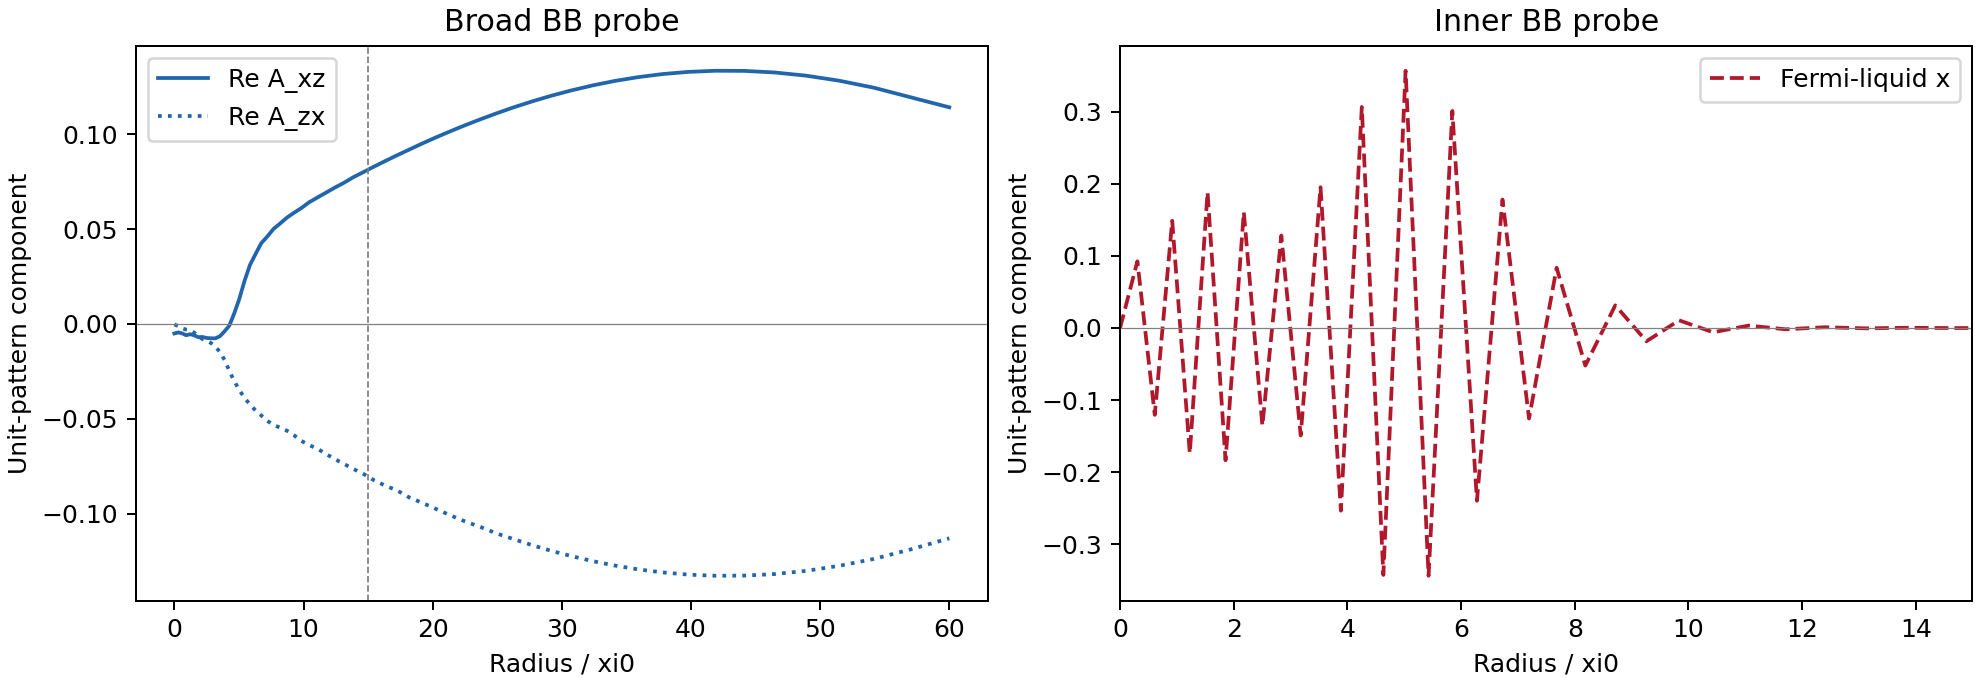
\includegraphics[width=\linewidth]{figures/signed_pattern_shapes.png}
\end{center}
Left: opposing off-diagonal components of the broad pattern. Right: magnified
$r\leq15\xi_0$, showing spatial sign alternation as well as localization.
This fine spatial structure should not be identified with a smooth physical
core mode without a refinement test.

\clearpage
\subsection{Evolution under BB and Anderson}
Project each method's \emph{unnormalized} residual onto the same two BB probes:
$q_j(k)=b_j^Tr_k$. These plots retain absolute decay, unlike projections of
unit residuals. They start at the first $E_{\max}\leq2\times10^{-5}$ crossing
and include all subsequent maps: BB 115--433, AA3 77--154, AA5 80--161,
AA10 91--224.
Windows have different lengths and do not represent identical states.
AA5 includes its repeated restart evaluation. BB-derived probes are a common
ruler, not a neutral basis optimised for each method.
\begin{center}
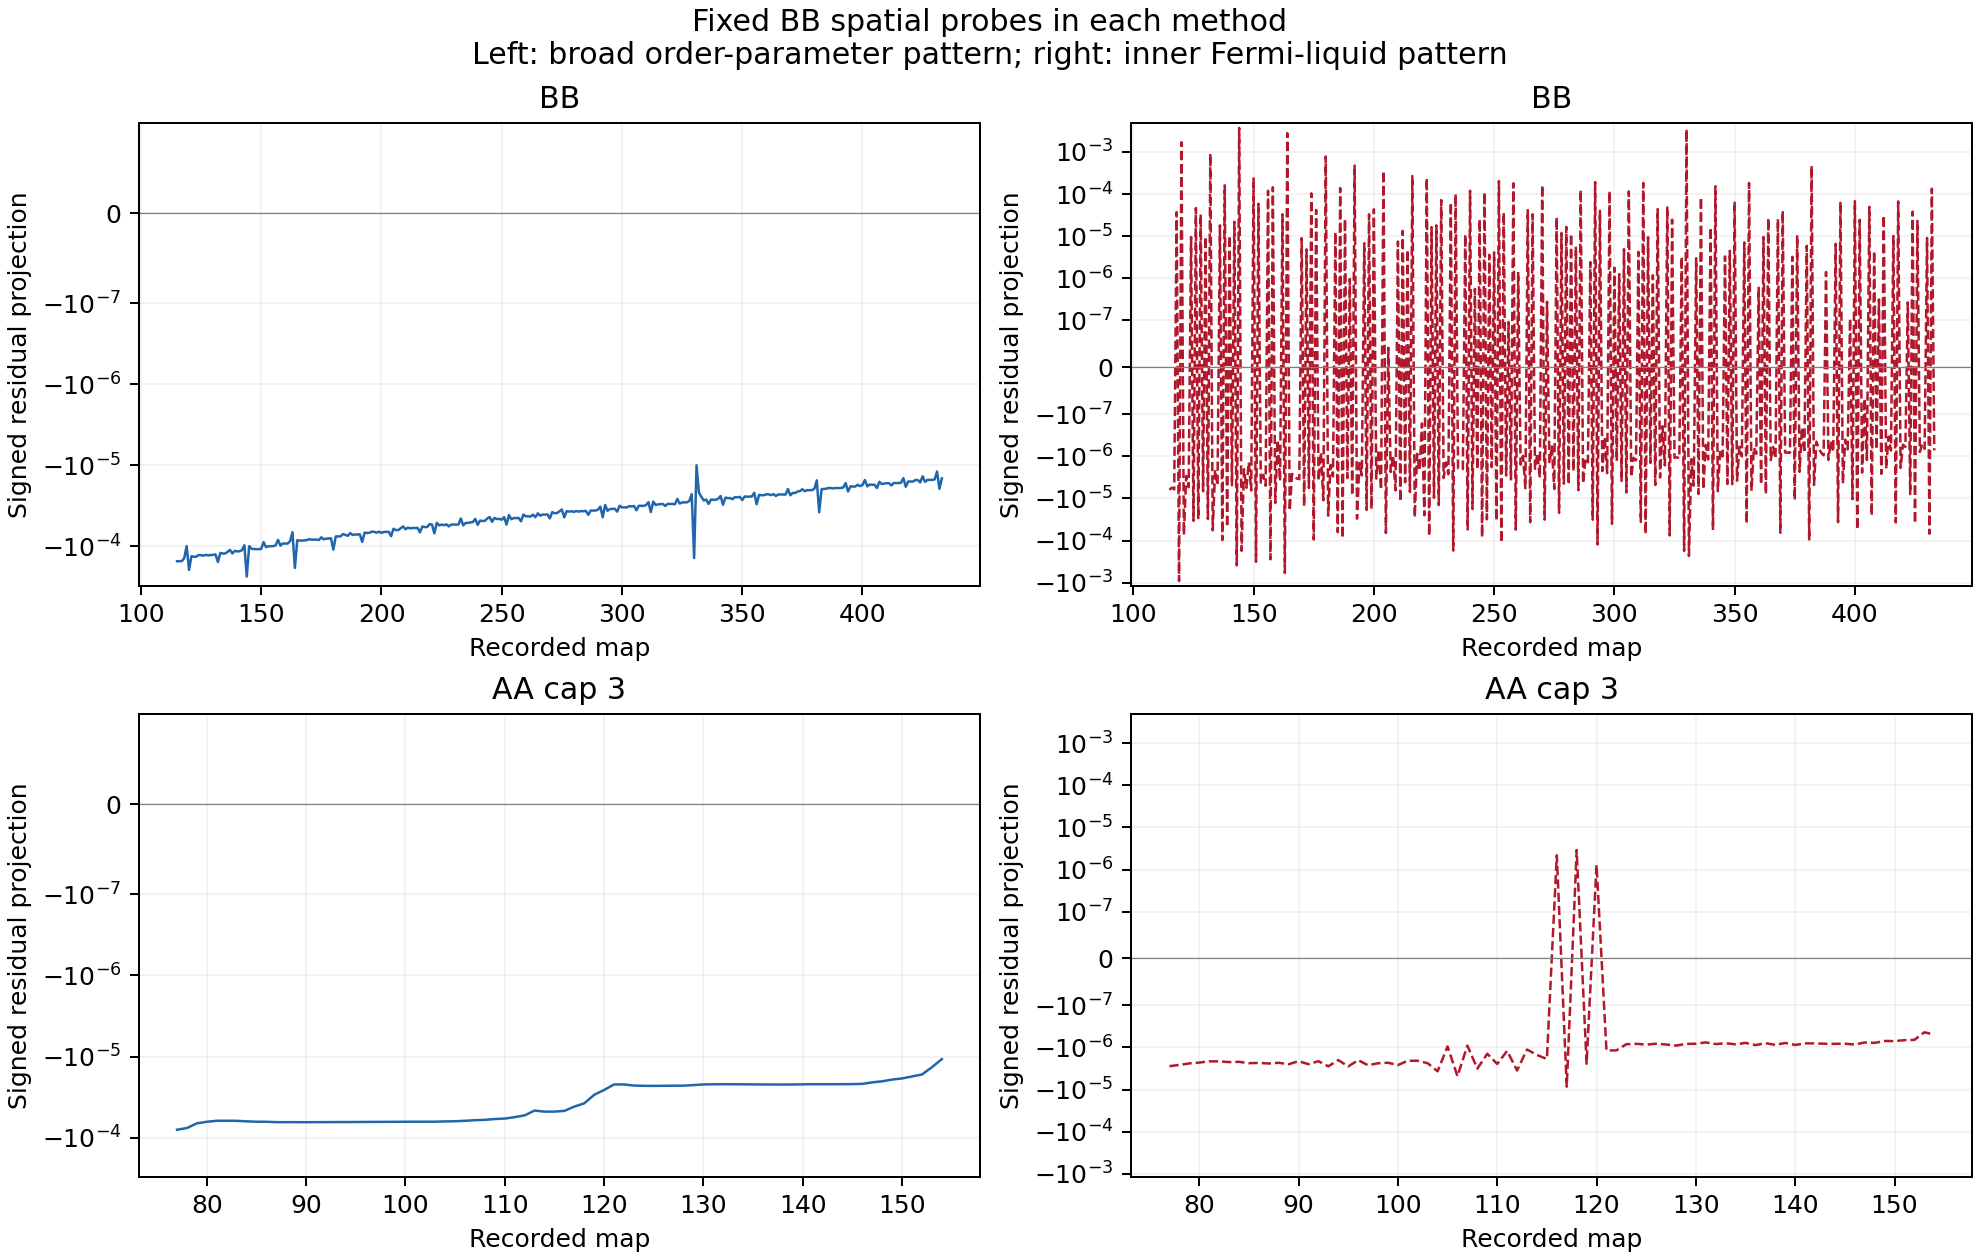
\includegraphics[width=\linewidth]{figures/signed_patterns_comparison_1.png}
\end{center}
\textbf{Reading the panels.} Left: the broad projection keeps its sign and
approaches zero, non-monotonically and at different rates. Right: the inner
projection repeatedly crosses zero, especially for BB. This is what
``oscillatory'' means here: iteration-to-iteration residual sign reversals.
Vertical scales match within each column across both figure pages and are
symmetric-logarithmic (linear for $|q|<10^{-7}$); horizontal ranges differ.
Inner projections are much smaller for Anderson, but
their sign changes have not disappeared.

\clearpage
\subsection{Signed histories for the larger Anderson caps}
The same fixed BB probes and vertical scales are used here. The dotted
vertical line marks AA5's restart; its first continuation evaluation repeats
the previously accepted state. Neither pattern is removed by Anderson.
\begin{center}
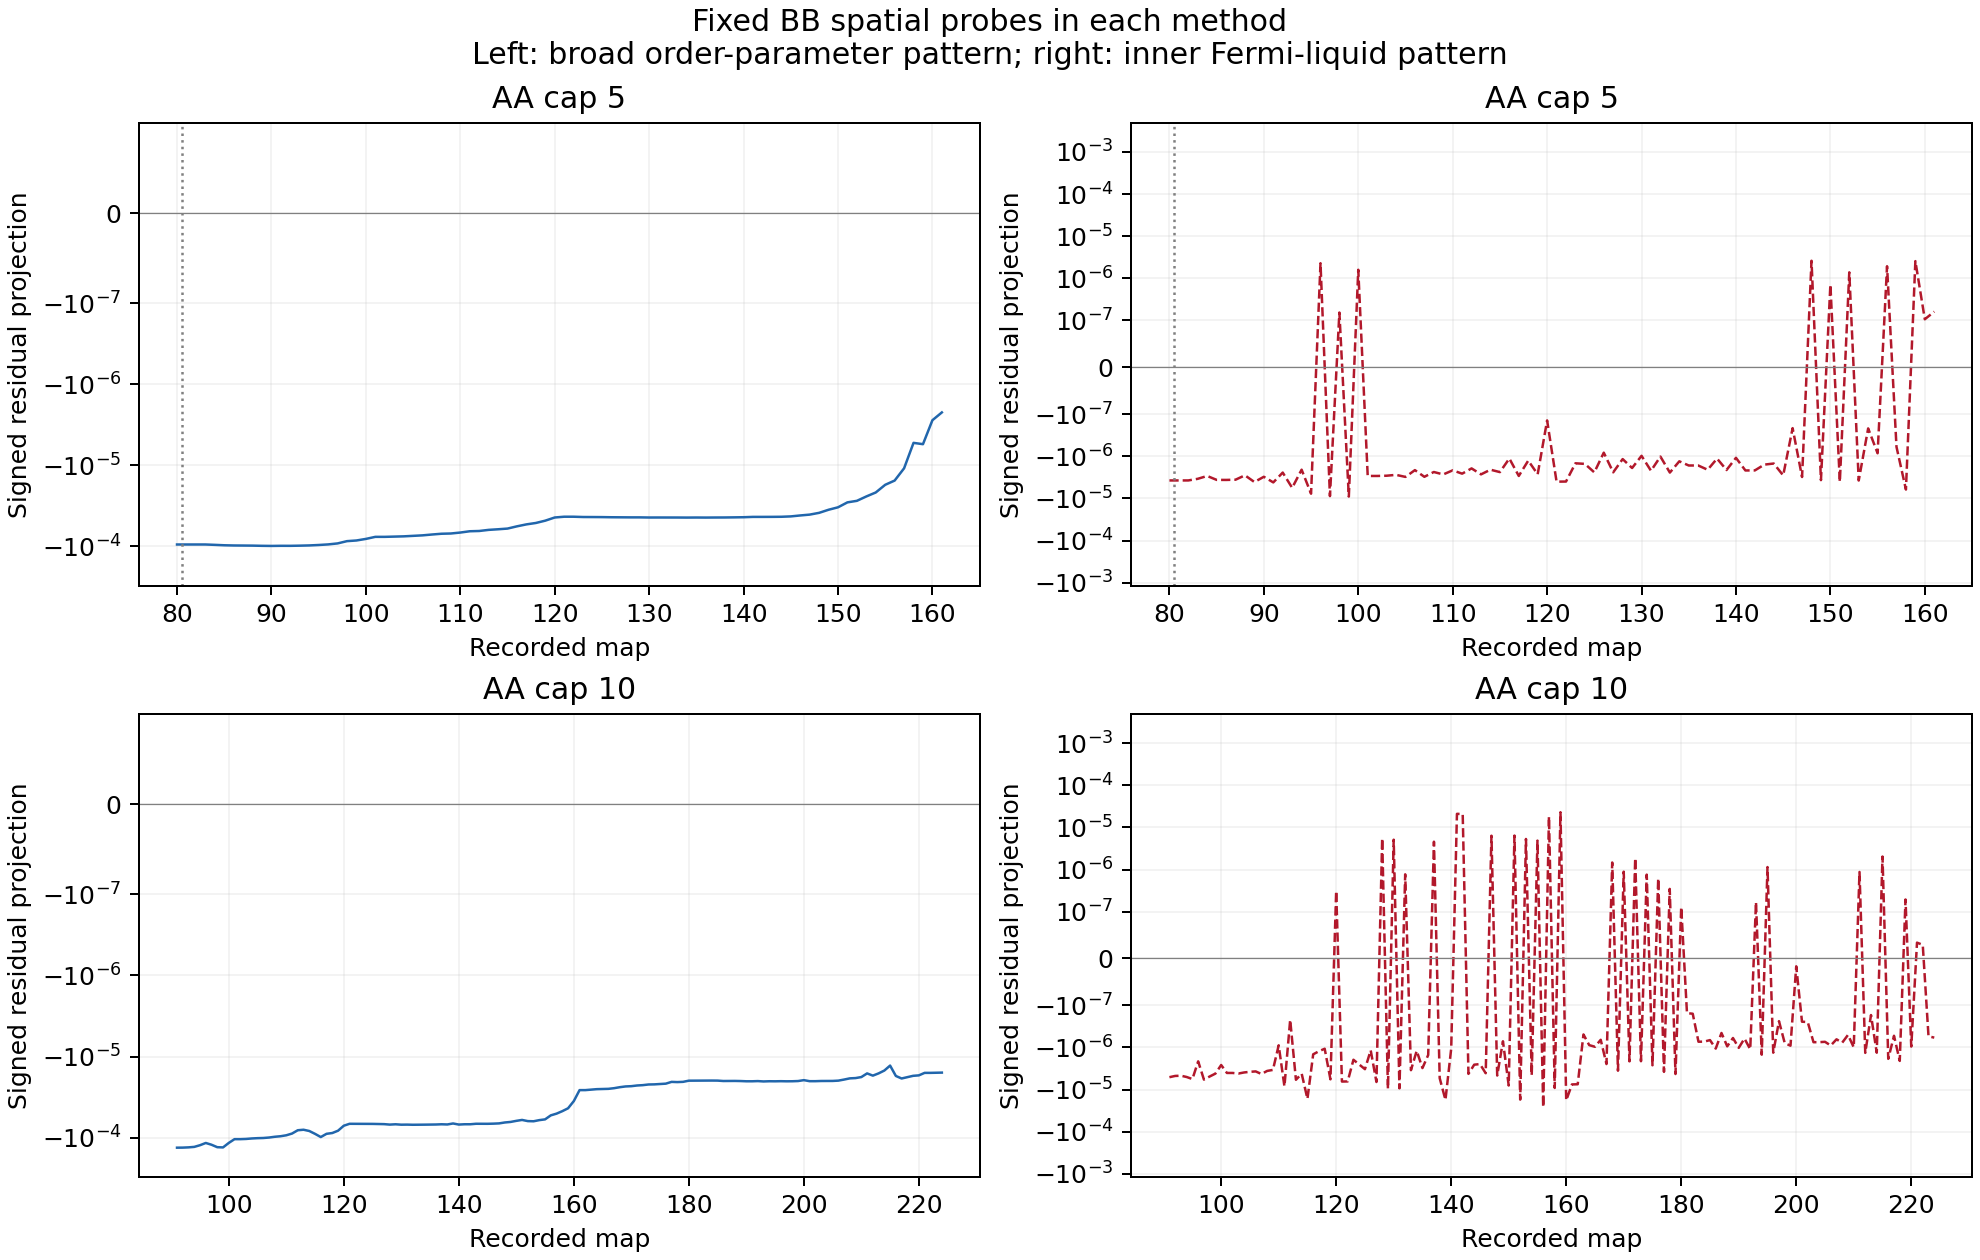
\includegraphics[width=\linewidth]{figures/signed_patterns_comparison_2.png}
\end{center}
The AA3 and AA5 inner projections are small relative to BB's, whereas AA10
has more visible excursions. These projections sample one fixed inner shape;
they do not include every possible spatial pattern of the inner residual.

\clearpage
\subsection{Independent checks of the Anderson tendencies}
To avoid relying only on a BB-derived basis, repeat the uncentred unit-residual
SVD independently for each method over the threshold-defined windows.
\begin{center}
\begin{tabular}{lrrrr}
\toprule
Diagnostic in threshold window & BB & AA3 & AA5 & AA10\\
\midrule
Leading-pattern squared-norm share &61.51\%&80.36\%&79.97\%&70.40\%\\
Leading pattern: outer rotation cosine &0.9957&0.9904&0.9969&0.9934\\
Mean share along fixed broad BB probe &61.17\%&78.41\%&78.50\%&70.13\%\\
Mean share along fixed inner BB probe &17.47\%&0.15\%&0.27\%&0.62\%\\
Inner BB-probe sign changes &234&6&15&50\\
Inner FL-vector reversals / pairs &227/318&54/77&66/81&104/133\\
\bottomrule
\end{tabular}
\end{center}
The mean fixed-probe share is
$\langle(b_j^Tr_k)^2/\|r_k\|^2\rangle_k$, not a physical energy.
``Inner FL'' includes all three Fermi-liquid components at $r\leq15\xi_0$;
a reversal means their consecutive-vector cosine is negative. Pattern shares
depend on window, scaling and normalization. The SVD percentages here differ
from the earlier maps-251--433 BB values for that reason.

All four independent leading patterns resemble the outer rotation tangent.
The rotation-like tendency is therefore not confined to BB. AA5's second
pattern is mixed (11.2\% in inner FL); AA10's second is mainly inner FL
(92.4\%), but carries only 4.37\% of unit-residual content. BB's second
carries 17.89\% and is 99.56\% inner FL in this window. AA3's second pattern
carries 6.59\% of unit-residual content and is predominantly outer (80.96\%),
with only 3.24\% in inner FL.

The inner FL subvector actually reverses frequently in all Anderson runs.
What is reduced is its weight in the \emph{whole} residual, not necessarily
its reversal frequency. A near-zero subvector can reverse without a large
change in global error. This explains why four and eighteen full-vector
reversals (and zero for AA3) do not imply an absence of inner oscillations. The fixed inner BB
probe samples only one spatial shape; other inner patterns may remain.

These observations are consistent with orientation adjustment of the soft
texture being a persistent numerical difficulty. They do not show that the
accelerator creates the soft core, that the physical texture is unstable,
or that iteration oscillations have a physical frequency. The earlier BB
spectral peaks near 6.31, 8.71 and 10.17 maps describe iteration history,
not an excitation spectrum or a single fixed clock.

\clearpage
\section{Comparison and conclusions for this benchmark}
\begin{center}
\begin{tabular}{lrrrrr}
\toprule
First maximum-error crossing & BB & Polyak & AA3 & AA5 & AA10\\
\midrule
$2\times10^{-4}$ &43&87&35&39&43\\
$2\times10^{-5}$ &115&319&77&80&91\\
$10^{-5}$ &172&517&105&107&128\\
$2\times10^{-6}$ &433&not reached&154&161&224\\
\bottomrule
\end{tabular}
\end{center}
\begin{center}
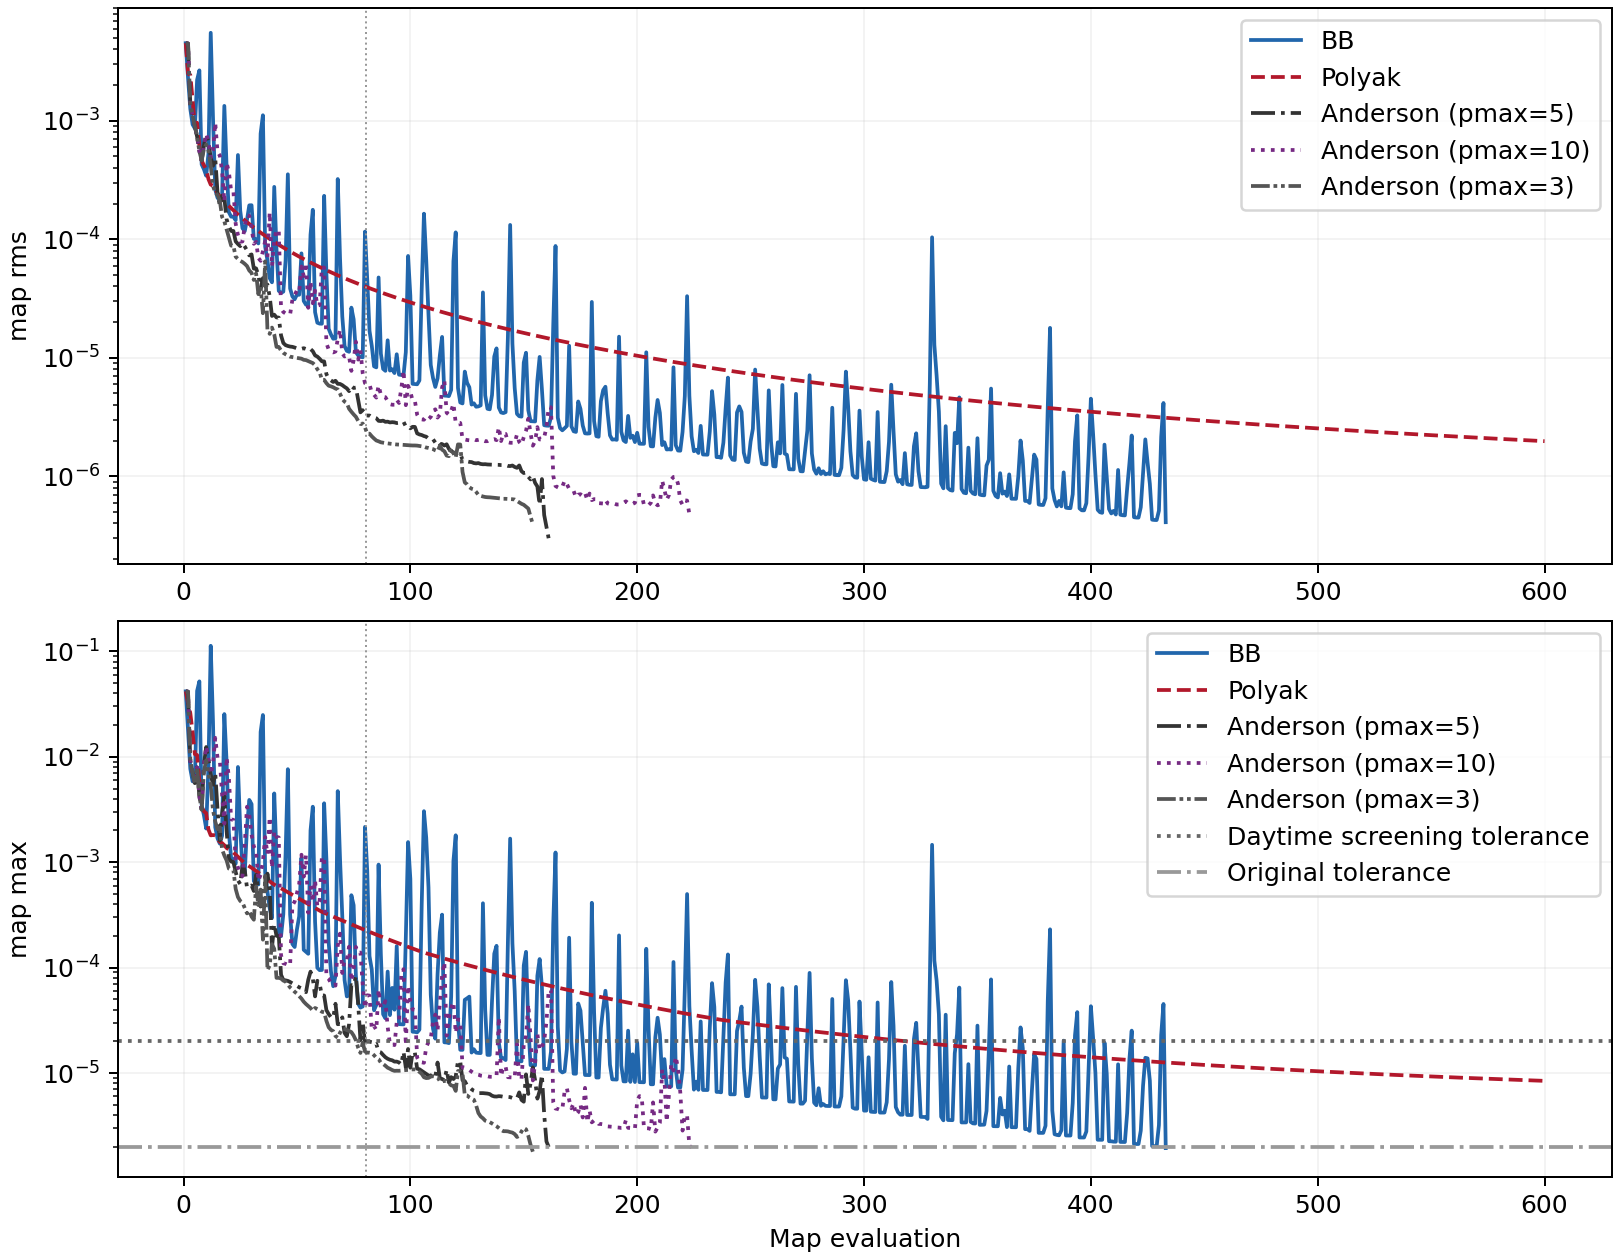
\includegraphics[width=.94\linewidth]{figures/accelerator_comparison.png}
\end{center}
AA3 has the fewest recorded maps of the tested settings: 154 versus 161 for
AA5 and 224 for AA10. The improvement over staged AA5 is modest (4.3\%);
AA3 also crosses the loose threshold first, before AA5's restart affects the
comparison. These samples do not establish an optimal cap. Polyak
has the smoothest RMS history but has not reached the tight tolerance.
This ranks these settings on this problem, not the algorithms universally.

Median map times are 17.34, 17.03, 17.08, 17.01 and 17.16 s for BB, Polyak,
AA3, AA5 and AA10. Summed AA map times are 2635, 2761 and 3851 s. BB has substantial timing
outliers, so total elapsed times are not controlled hardware measurements.
AA5's staged execution remains a caveat; a tight single-segment control would
remove it. AA3 is the best observed cap here, not a demonstrated universal optimum.

Structured residuals suggest testing history/reset policies and spatial
resolution before invoking a numerical noise floor or removing a presumed
zero mode. Physical hard/soft-core structure is the background to this
interpretation, not something inferred solely from these residual plots.

\clearpage
\section{Data provenance and reproduction}
All directories below are relative to the FermiForge project root.
\begin{lstlisting}
runs/261001-192802-radial-bb-diagnostics-0plus-T030-Fs54-radial-reference
runs/261001-233335-radial-polyak-scratch-0plus-T030-Fs54-radial-reference
runs/261002-091852-radial-anderson-aa20-diagnostics-0plus-T030-Fs54-radial-reference
runs/261002-094542-radial-anderson-aa20-0plus-pmax5-tight-continuation-radial-reference
runs/261002-111709-radial-anderson-aa20-0plus-pmax10-scratch-T030-Fs54-radial-reference
runs/261002-130520-radial-anderson-aa20-0plus-pmax3-scratch-T030-Fs54-radial-reference
\end{lstlisting}
Input namelists, metrics, histories, signed vectors and manifests are primary
records. Signed layout is block-major: real and imaginary parts of
$A_{xx},A_{xy},\ldots,A_{zz}$, then three Fermi-liquid fields; each block
has 60 nodes. Matrix indices are spin then orbital. No solver or archived
run data were changed by this analysis.

To reproduce figures and numerical summaries:
\begin{lstlisting}
python3 tools/analyze_signed_radial_bb.py \
  runs/261001-192802-radial-bb-diagnostics-0plus-T030-Fs54-radial-reference
python3 tools/compare_radial_accelerators.py
python3 tools/compare_signed_residual_patterns.py
cd docs/technical_note
pdflatex -interaction=nonstopmode accelerator_diagnostics.tex
\end{lstlisting}
Machine-readable summaries are retained in \path{work/signed-bb-analysis/}:
\begin{lstlisting}
analysis.json
accelerator_comparison.json
signed_pattern_comparison.json
\end{lstlisting}
Figures are retained beside the source: compilation does not require raw
data; regeneration needs the archived runs, NumPy and Matplotlib.

Scratch launchers create new dated outputs and start solver runs; they are
not part of document reproduction:
\begin{lstlisting}
bash tools/run_radial_anderson_diagnostics.sh 0plus --tolerance 2e-6
bash tools/run_radial_anderson_p10.sh
bash tools/run_radial_anderson_p3.sh
\end{lstlisting}
\begin{thebibliography}{9}
\bibitem{superconga}
P. Holmvall et al., \emph{SuperConga: An open-source framework for mesoscopic
superconductivity}, Applied Physics Reviews \textbf{10}, 011317 (2023),
doi:10.1063/5.0100324. Appendix E supplies the Polyak recurrence and defaults.
\end{thebibliography}
\end{document}
